\documentclass{article}
\PassOptionsToPackage{numbers,compress}{natbib}
\usepackage[final]{neurips_2020}
\makeatletter
\renewcommand{\@noticestring}{SYDE 522 Fundamentals of AI, Final Project. University of Waterloo, Fall 2026.}
\makeatother
\usepackage[utf8]{inputenc}
\usepackage[T1]{fontenc}
\usepackage[hidelinks]{hyperref}
\usepackage{url}
\usepackage{booktabs}
\usepackage{amsfonts,amsmath}
\usepackage{nicefrac}
\usepackage{microtype}
\usepackage{graphicx}

\title{Linear Models, Kernel SVMs and MLPs\\ on the UCI Letter Recognition Task}

\author{%
  Mira Suthakar \\
  University of Waterloo \\
  Waterloo, ON, Canada \\
  \And
  Tharun [last name] \\
  University of Waterloo \\
  Waterloo, ON, Canada \\
}

\begin{document}
\maketitle

\begin{abstract}
We study 26-class letter recognition on the UCI Letter Recognition dataset (20,000 examples, 16 integer features) and ask how much nonlinearity the task requires. We compare methods from the course: ordinary and ridge least squares, logistic regression, the perceptron, SVMs with linear, polynomial and RBF kernels, and multilayer perceptrons (MLPs) of three sizes. For each, we vary regularization, kernel and architecture hyperparameters on a validation set, then report test accuracy once, with bootstrap confidence intervals. Linear classifiers reach only 51--84\% test accuracy, whereas an RBF-kernel SVM reaches 97.4\% and the larger MLPs about 95\%. Ridge regression is identical to ordinary least squares on the raw features (54.7\%) but reaches 92.8\% after an explicit cubic feature expansion, an explicit counterpart of the kernel trick. The SVM beats the best MLP by 2.2 points (95\% CI 1.7 to 2.7) at lower training cost.
\end{abstract}

\section{Introduction}
Many classical results in machine learning concern when a linear model is enough and when it is not. Our goal is to see this on one concrete task: predicting which capital letter of the English alphabet a small image shows, from 16 numerical summaries of the image. The dataset is clean and balanced, so differences between methods reflect model capacity and tuning rather than data problems. Our hypothesis is that the classes are not linearly separable in this feature space, so linear methods should plateau well below kernel methods and neural networks.

We compare five method families (eleven final models), choose hyperparameters on held-out validation data, and evaluate on a test set used once. For every method, we vary the hyperparameters that control its flexibility and regularization and report validation accuracy, so that the paper shows what we did, why, and what happened. We also study training-set size, the effect of exact duplicate examples, and the letters that are confused.

\section{Task and dataset}
\paragraph{Task.} Multi-class classification with 26 classes (A to Z). The metric is accuracy, supported by macro-averaged F1, confusion matrices and fit time.

\paragraph{Data.} We use the UCI Letter Recognition dataset \citep{frey1991letter,dua2019uci}, available on Kaggle as \texttt{letter-recognition.csv}. Black-and-white rectangular images of capital letters were generated from 20 fonts, with each letter randomly distorted, giving 20,000 stimuli. Each image was converted into 16 primitive integer attributes (statistical moments and edge counts, such as box position and size, number of ``on'' pixels, mean pixel positions, variances and correlations, and edge counts) scaled to the integers 0 to 15. There are no missing values, so no imputation or feature engineering is needed. The classes are nearly balanced, with 734 to 813 examples per letter (Figure~\ref{fig:data}), so accuracy is a fair headline metric. The original authors report a little over 80\% accuracy with Holland-style classifier systems \citep{frey1991letter}.

\begin{figure}[t]
  \centering
  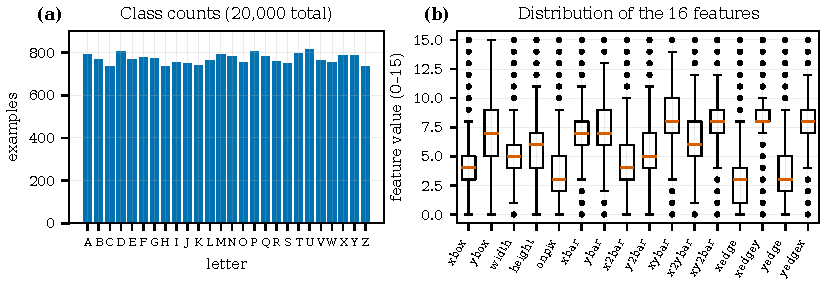
\includegraphics[width=\linewidth]{figures/fig1_data.pdf}
  \caption{The dataset. (a) Examples per letter: the classes are nearly balanced. (b) Distribution of each of the 16 integer features, which share a 0--15 scale.}
  \label{fig:data}
\end{figure}

\paragraph{Duplicates.} Because the features are coarse integers, distinct images can map to the same feature vector: 1,332 rows are exact duplicates of another row (feature vector and label), and 380 of the 4,000 test examples also appear in the training pool. Every duplicated feature vector has a single label. We keep the standard split for the main results and also report accuracy on the 3,620 test examples that do not appear in training (``no-overlap'' in Table~\ref{tab:final}).

\section{Methods and rationale}
We chose methods that span a range of capacity, from a linear model with one weight matrix to a kernel machine and deep networks, so that we could see where accuracy stops improving. Table~\ref{tab:hyper} lists the hyperparameters varied for each method.

\paragraph{Least squares and ridge regression.} The simplest baseline: each letter becomes a one-hot vector of length 26, we fit a linear map by least squares, and predict the letter with the largest output. Ridge regression \citep{hoerl1970ridge} adds an L2 penalty $\alpha\lVert W\rVert^2$; we vary $\alpha$ to test whether shrinkage helps. To test whether the linear hypothesis class is the bottleneck, we also fit ridge on explicit polynomial expansions of the standardized features (degree 2: 152 features; degree 3: 968), the explicit counterpart of a polynomial kernel.

\paragraph{Logistic regression.} Multinomial (softmax) regression has linear decision boundaries like least squares but a probabilistic loss. We vary the inverse regularization strength $C$ and the penalty type (L1 or L2).

\paragraph{Perceptron.} Rosenblatt's perceptron \citep{rosenblatt1958perceptron}, as 26 one-vs-rest binary classifiers. It is the classic simple linear classifier and is guaranteed to converge only on separable data, so we vary the number of epochs. We also vary the learning rate $\eta$; since weights start at zero, scaling $\eta$ only rescales the weights and should not change predictions, which we check.

\paragraph{Support vector machines.} Maximum-margin classifiers with soft margins \citep{cortes1995support}, using LIBSVM's one-vs-one multi-class scheme \citep{chang2011libsvm}. With kernel $k(x,x')$ the model needs only inner products between examples, which is the kernel trick \citep{boser1992training}. We compare the linear kernel, the polynomial kernel (degree $d$, $k=(\gamma\, x^\top x'+1)^d$) and the RBF kernel $k=\exp(-\gamma\lVert x-x'\rVert^2)$. $C$ trades margin width against training errors; $\gamma$ sets the RBF width (large $\gamma$ is more flexible); $d$ sets polynomial complexity. The cost is an $N\times N$ kernel matrix, which is comfortable at $N\approx 10^4$.

\paragraph{Multilayer perceptrons.} Fully connected networks with ReLU units and a softmax output, trained by back-propagation \citep{rumelhart1986learning} with the Adam optimizer \citep{kingma2015adam}, mini-batches of 200 and cross-entropy loss; training stops after 150 epochs or when the loss has not improved by $10^{-4}$ for 10 epochs. We define three architectures: \emph{simple} (one hidden layer of 16 units), \emph{medium} (two layers of 64) and \emph{deep} (four layers of 128). We vary depth, width, learning rate, L2 penalty and number of epochs, because these control capacity, optimization speed and overfitting.

\begin{table}[t]
  \caption{Hyperparameters varied for each method, and why.}
  \label{tab:hyper}
  \centering
  \footnotesize
  \begin{tabular}{@{}p{0.17\linewidth}p{0.45\linewidth}p{0.33\linewidth}@{}}
    \toprule
    Method & Varied (values) & Reason \\
    \midrule
    OLS / ridge & $\alpha\in\{10^{-3},\dots,10^{5}\}$ (9 values); polynomial degree 1, 2, 3 & bias--variance trade-off; is the linear class the bottleneck? \\
    Logistic reg. & $C\in\{10^{-4},\dots,10^{3}\}$; L1 or L2 penalty & strength and form of regularization \\
    Perceptron & epochs 1 to 200 (5 seeds); $\eta\in\{0.01,\dots,100\}$ & convergence on non-separable data \\
    SVM, linear & $C\in\{10^{-3},\dots,10\}$ & margin vs.\ training errors \\
    SVM, poly. & degree 2, 3, 4; $C\in\{1,10\}$ & implicit polynomial features \\
    SVM, RBF & $C\in\{0.1,\dots,1000\}$ $\times$ $\gamma\in\{10^{-3},\dots,1\}$ (35 pairs) & margin and kernel width \\
    MLP & depth 1--4 $\times$ width 16--128; learning rate $10^{-4}$ to $3{\cdot}10^{-2}$; L2 $\alpha\in\{0,\dots,1\}$; epochs (curves to 100) & capacity, optimization, regularization, early stopping \\
    \bottomrule
  \end{tabular}
\end{table}

\section{Experimental protocol}
\paragraph{Data splits.} Following the UCI convention, the first 16,000 examples form the training pool and the last 4,000 the test set, which is not touched until every hyperparameter has been chosen. For tuning, we split the pool at random (fixed seed) into 12,000 training and 4,000 validation examples; every sweep trains on the 12,000 and is scored on the validation examples. Features are standardized with statistics computed on the training data only. For each method, the setting with the highest validation accuracy is selected (ties go to the more regularized or simpler setting), the model is retrained on all 16,000 pool examples, and test accuracy is computed once. Stochastic methods (perceptron, MLP) use five random seeds.

\paragraph{Uncertainty.} We give 95\% bootstrap confidence intervals for test accuracy (1,000 resamples of the 4,000 test examples, averaging over seeds for stochastic models) and paired bootstrap intervals for differences between models. A validation accuracy on 4,000 examples has a standard error of about 0.3 points, so validation differences below about 0.7 points should not be over-interpreted.

\paragraph{MLP tuning.} Depth and width are swept on a grid with the default learning rate ($10^{-3}$) and penalty ($10^{-4}$). Learning rate and penalty are then swept one at a time on the medium network; the best pair (0.01, 0.1) improved validation accuracy over the defaults (94.8\% vs.\ 94.5\%) and is used for all three architectures. Experiments use scikit-learn \citep{pedregosa2011scikit} on a single CPU core.

\section{Results}
\subsection{Linear models, and linear models on polynomial features}
\begin{figure}[t]
  \centering
  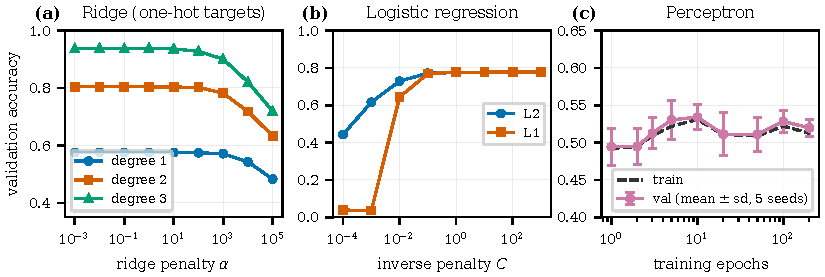
\includegraphics[width=\linewidth]{figures/fig2_simple.pdf}
  \caption{Validation accuracy of the simple models. (a) Ridge regression with one-hot targets for polynomial degrees 1 to 3. (b) Logistic regression for L1 and L2 penalties. (c) Perceptron versus epochs (mean $\pm$ s.d.\ over 5 seeds).}
  \label{fig:simple}
\end{figure}
Least squares reaches only 54.7\% test accuracy (Table~\ref{tab:final}), and ridge regression is indistinguishable from it (paired difference 0.0 points, CI $-$0.1 to 0.1). Figure~\ref{fig:simple}a shows why: validation accuracy is flat (57.5 to 57.6\%) for $\alpha\le 100$ and falls for larger $\alpha$. Training accuracy is only 56\%, so the model underfits, and with 16 features and 12,000 examples there is no variance for shrinkage to remove. Raising the capacity changes this completely: ridge on degree-2 features reaches 80.4\% validation accuracy and on degree-3 features (968 features) 93.8\% (92.8\% test), again flat for $\alpha\le 10$. The failure of the linear model is therefore a failure of its hypothesis class, not of the loss or the regularization.

Logistic regression does better than least squares (77.3\% test), but it saturates quickly: validation accuracy rises from 44\% at $C=10^{-4}$ to 77.7\% at $C\ge10$, L1 and L2 agree for $C\ge1$, and L1 with $C\le10^{-3}$ predicts at chance level, presumably because the penalty drives all weights to zero (Figure~\ref{fig:simple}b). The perceptron is the weakest method at 50.8\% test accuracy. Its validation accuracy hovers between 49\% and 53\% for any number of epochs, with run-to-run standard deviations of 1 to 3 points (Figure~\ref{fig:simple}c), because the data are not linearly separable and the algorithm never converges. As predicted, the learning rate has no effect: predictions are identical for $\eta$ from 0.01 to 100.

\subsection{Support vector machines}
\begin{figure}[t]
  \centering
  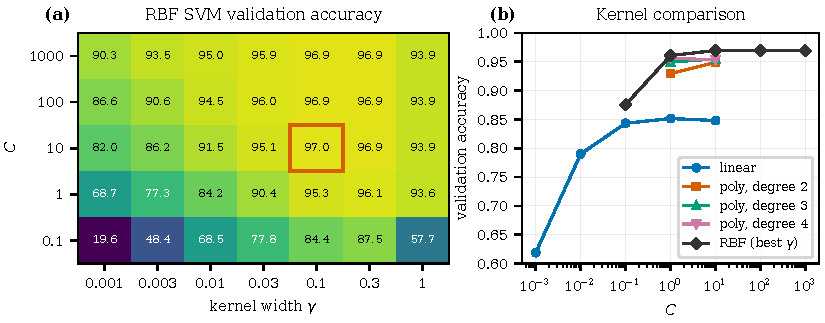
\includegraphics[width=\linewidth]{figures/fig3_svm.pdf}
  \caption{SVM validation accuracy. (a) RBF kernel over a grid of $C$ and $\gamma$ (outlined: selected). (b) Best accuracy per $C$ for each kernel.}
  \label{fig:svm}
\end{figure}
The linear-kernel SVM improves with $C$ from 61.9\% to 85.2\% validation accuracy and is flat beyond $C=1$ (84.0\% test). It clearly beats logistic regression and the perceptron, possibly in part because one-vs-one decomposition only has to separate pairs of letters. Polynomial kernels close most of the gap: at $C=1$, degrees 2, 3 and 4 give 92.9\%, 95.0\% and 95.7\% validation accuracy (selected: degree 4, 96.4\% test).

The RBF kernel is the most accurate and also the most sensitive to its two hyperparameters (Figure~\ref{fig:svm}a): validation accuracy ranges from 19.6\% ($C=0.1$, $\gamma=0.001$, an almost flat decision function) to 97.0\% ($C=10$, $\gamma=0.1$). Good settings lie along a diagonal, where a larger $\gamma$ compensates for a smaller $C$. A very large $\gamma=1$ is worse (93.9\%) because the kernel becomes too narrow. The selected model uses 5,881 of the 12,000 training examples as support vectors and reaches 97.4\% test accuracy (95\% CI 96.9 to 97.9).

\subsection{Multilayer perceptrons}
\begin{figure}[t]
  \centering
  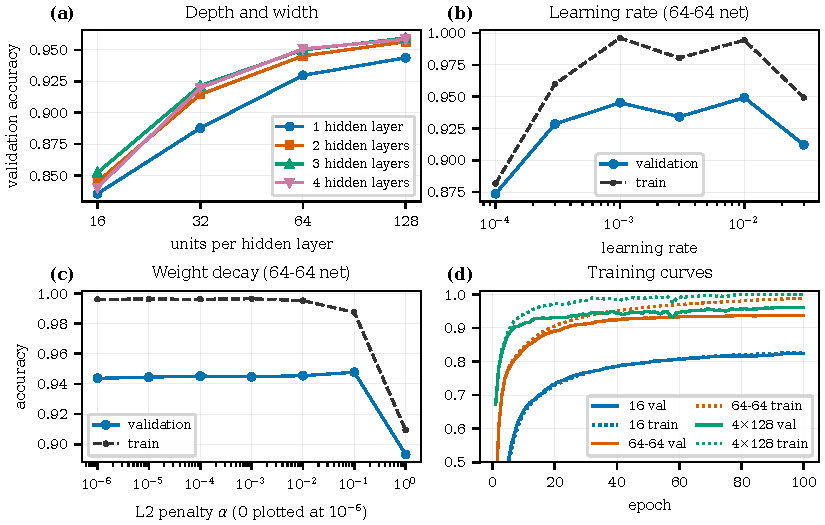
\includegraphics[width=\linewidth]{figures/fig4_mlp.pdf}
  \caption{MLP validation accuracy. (a) Depth and width. (b) Learning rate and (c) L2 penalty for the 64-64 network. (d) Training curves (default settings) for three architectures.}
  \label{fig:mlp}
\end{figure}
Capacity matters a great deal at small widths (Figure~\ref{fig:mlp}a): a single hidden layer of 16 units reaches 83.6\% and one of 128 units 94.4\%. Adding a second layer helps at widths of 64 and above (93.0\% to 94.5\% at 64 units; 94.4\% to 95.7\% at 128 units), but layers beyond two change validation accuracy by 0.7 points or less, within the noise level. The learning rate matters (Figure~\ref{fig:mlp}b): $10^{-4}$ underfits (87.4\%, still improving after 150 epochs) and $3\times10^{-2}$ is too large (91.2\%), while $10^{-2}$ is best (94.9\%). The L2 penalty has little effect up to 0.01, is mildly helpful at 0.1 (94.8\%, training accuracy 98.8\% instead of 99.6\%) and underfits at 1 (89.3\%). The training curves (Figure~\ref{fig:mlp}d) show a small network that underfits (82.8\% training accuracy after 100 epochs) and larger ones that fit the training set almost perfectly (98.9\% and 100\% at epoch 100). Validation accuracy of the medium network levels off at about 93.7\% after roughly 80 epochs, and that of the deep network is still creeping up (96.1\% at epoch 100); neither declines, so overfitting shows up as a train--validation gap rather than as falling validation accuracy.

\subsection{Training-set size and final comparison}
\begin{figure}[t]
  \centering
  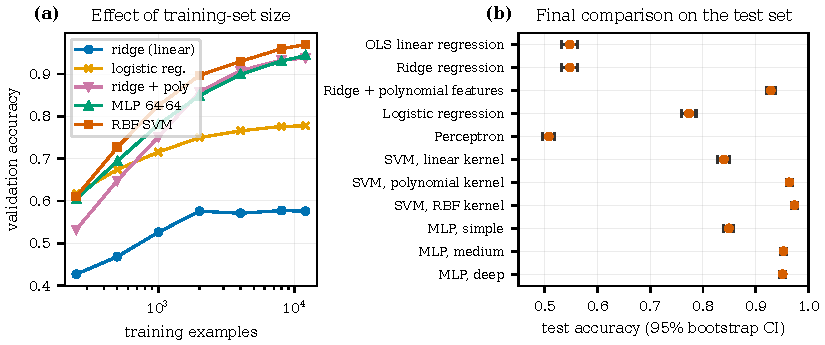
\includegraphics[width=\linewidth]{figures/fig5_final.pdf}
  \caption{(a) Validation accuracy as the training set grows (best settings from the 12,000-example sweeps, not retuned; MLP: mean of 3 seeds). (b) Test accuracy with 95\% bootstrap confidence intervals.}
  \label{fig:final}
\end{figure}
Figure~\ref{fig:final}a shows how the methods use data. Linear least squares is flat at about 57\% beyond 2,000 examples and logistic regression saturates at about 78\%, whereas ridge with polynomial features, the MLP and the RBF SVM keep improving up to 12,000 examples (the SVM from 61\% at 250 examples to 97\%). With very little data the picture reverses: at 250 examples logistic regression (61.8\%) matches the SVM (61.1\%) and the MLP (60.4\%), although the hyperparameters were not retuned for each size.

Table~\ref{tab:final} and Figure~\ref{fig:final}b give the final test results. The ordering by test accuracy is RBF SVM $>$ polynomial SVM $>$ MLPs $>$ ridge with cubic features $>$ linear SVM $\approx$ simple MLP $>$ logistic regression $>$ least squares/ridge $>$ perceptron. The RBF SVM beats the MLP with the highest validation accuracy (deep) by 2.2 points (paired 95\% CI 1.7 to 2.7), the polynomial SVM by 0.95 (0.55 to 1.35), and ridge with cubic features by 4.5 (3.8 to 5.2). The medium and deep MLPs are statistically indistinguishable (difference 0.1 points, CI $-$0.2 to 0.5), while both beat the simple MLP by about 10 points. Macro-F1 tracks accuracy closely, as expected with balanced classes. Excluding test examples that also occur in training lowers accuracy by 0.3 to 2.3 points (logistic regression 77.3\% to 75.4\%; RBF SVM 97.4\% to 97.1\%) without changing the ranking. The RBF SVM also trained faster (1.9 s) than the medium (4.6 s) and deep (20.3 s) MLPs on this CPU.

\begin{table}[t]
  \caption{Final results. Val.\ is validation accuracy at the selected setting (\%); test accuracy is on the 4,000 held-out examples (mean over 5 seeds for the perceptron and MLPs, s.d.\ 1.2, 0.4, 0.3 and 0.6 points for the perceptron and the simple, medium and deep MLPs). All MLPs use learning rate 0.01 and L2 penalty 0.1. ``No-overlap'' is accuracy on the 3,620 test examples absent from training. Fit time is for 16,000 examples.}
  \label{tab:final}
  \centering
  \footnotesize
  \setlength{\tabcolsep}{3.5pt}
  \begin{tabular}{@{}llccccc@{}}
\toprule
Model & Selected setting & Val. & Test acc. [95\% CI] & Macro-F1 & No-overlap & Fit (s) \\
\midrule
OLS linear regression & -- & 57.6 & 54.7 [53.1, 56.1] & 51.2 & 52.4 & <0.1 \\
Ridge regression & $\alpha{=}10$ & 57.6 & 54.7 [53.1, 56.1] & 51.1 & 52.4 & <0.1 \\
Ridge + polynomial features & degree 3, $\alpha{=}1$ & 93.8 & 92.8 [92.1, 93.7] & 92.9 & 92.2 & 0.4 \\
\midrule
Logistic regression & L2, $C{=}10$ & 77.7 & 77.3 [75.9, 78.7] & 77.2 & 75.4 & 0.4 \\
Perceptron & 10 epochs & 53.4 & 50.8 [49.6, 51.9] & 50.6 & 49.2 & 0.2 \\
\midrule
SVM, linear kernel & $C{=}1$ & 85.2 & 84.0 [82.7, 85.1] & 84.0 & 82.4 & 2.3 \\
SVM, polynomial kernel & degree 4, $C{=}1$ & 95.7 & 96.4 [95.8, 97.0] & 96.4 & 96.0 & 1.4 \\
SVM, RBF kernel & $C{=}10$, $\gamma{=}0.1$ & 97.0 & \textbf{97.4} [96.9, 97.9] & 97.4 & 97.1 & 1.9 \\
\midrule
MLP, simple & 1$\times$16 & 85.5 & 84.9 [83.9, 85.8] & 85.0 & 83.5 & 3.7 \\
MLP, medium & 2$\times$64 & 94.3 & 95.3 [94.8, 95.8] & 95.3 & 94.8 & 4.6 \\
MLP, deep & 4$\times$128 & 94.4 & 95.1 [94.6, 95.6] & 95.1 & 94.7 & 20.3 \\
\bottomrule
\end{tabular}

\end{table}

\subsection{Errors}
\begin{figure}[t]
  \centering
  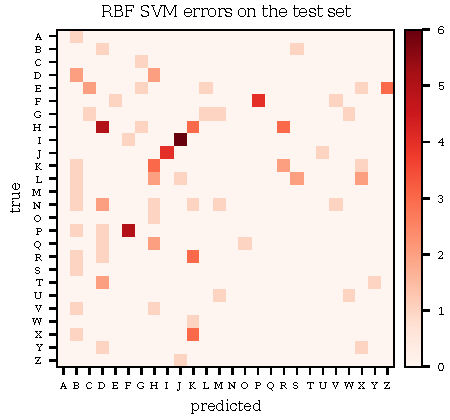
\includegraphics[width=0.52\linewidth]{figures/fig6_confusion.pdf}
  \caption{Test errors of the RBF SVM (106 of 4,000); diagonal removed.}
  \label{fig:conf}
\end{figure}
The RBF SVM makes only 106 errors on the test set, spread over many pairs of letters (Figure~\ref{fig:conf}). The most frequent confusions are between visually similar letters: I and J (10 errors in both directions), P and F (9), H as D (5), and X and R predicted as K, and K as H (3 each).

\section{Discussion}
\paragraph{Nonlinearity is essential, and kernels provide it cheaply.} Every linear classifier we tried reached at most 84\% test accuracy, and every nonlinear model with enough capacity reached at least 92.8\% (the 16-unit MLP, at 84.9\%, is the exception). Ridge with cubic features shows that the missing ingredient is the feature map rather than a better loss: the 968-dimensional expansion nearly closes the gap. A kernel provides such a map implicitly. The polynomial and RBF SVMs beat the explicit expansion by 3.6 and 4.5 points with $16$-dimensional inputs and no expansion to store.

\paragraph{SVM versus MLP.} The RBF SVM was about two points better than the MLPs, which is consistent with kernel methods being strong on moderate-size, low-dimensional problems like this one. This comparison favours the SVM in one respect: it received a 35-point joint grid over $C$ and $\gamma$, while the MLPs were tuned one hyperparameter at a time, so more MLP tuning (batch size, activations, learning-rate schedules) could narrow the gap.

\paragraph{Limitations.} All tuning used a single train/validation split. We used scikit-learn defaults for some choices (ReLU, Adam, batch size 200) and coarse logarithmic grids. Test confidence intervals are about $\pm0.5$ points, so only the larger gaps in Table~\ref{tab:final} are reliable. Duplicate feature vectors inflate all test accuracies slightly. The dataset has only 20 fonts, so the results say little about handwriting or other scripts.

\section{Conclusion}
On the letter recognition task, linear models are limited to 51--84\% test accuracy, polynomial features or a kernel bring the same linear machinery above 92\%, and an RBF-kernel SVM is best at 97.4\%, ahead of tuned MLPs at about 95\%. Hyperparameters matter most for the flexible models: accuracy of the RBF SVM varied between 20\% and 97\% across $(C,\gamma)$, and MLP accuracy between 84\% and 96\% across sizes, while moderate regularization made no difference for the linear models and strong regularization only hurt.

\section*{Broader Impact}
Letter recognition from clean, balanced, synthetic distortions of 20 fonts is a benign benchmark. The main risk is over-generalizing these results to handwriting or other scripts, where errors could affect people (for example, in automated form reading); no such evaluation was done here.

\small
\bibliographystyle{plainnat}
\begin{thebibliography}{99}
\bibitem[Boser et~al.(1992)]{boser1992training} B.~E. Boser, I.~M. Guyon, and V.~N. Vapnik. A training algorithm for optimal margin classifiers. In \emph{Proc.\ Fifth Annual Workshop on Computational Learning Theory}, pages 144--152, 1992.
\bibitem[Chang and Lin(2011)]{chang2011libsvm} C.-C. Chang and C.-J. Lin. LIBSVM: a library for support vector machines. \emph{ACM Trans.\ Intelligent Systems and Technology}, 2(3):27, 2011.
\bibitem[Cortes and Vapnik(1995)]{cortes1995support} C.~Cortes and V.~Vapnik. Support-vector networks. \emph{Machine Learning}, 20(3):273--297, 1995.
\bibitem[Dua and Graff(2019)]{dua2019uci} D.~Dua and C.~Graff. UCI Machine Learning Repository, 2019. \url{https://archive.ics.uci.edu/dataset/59/letter+recognition}.
\bibitem[Frey and Slate(1991)]{frey1991letter} P.~W. Frey and D.~J. Slate. Letter recognition using Holland-style adaptive classifiers. \emph{Machine Learning}, 6(2):161--182, 1991.
\bibitem[Hoerl and Kennard(1970)]{hoerl1970ridge} A.~E. Hoerl and R.~W. Kennard. Ridge regression: biased estimation for nonorthogonal problems. \emph{Technometrics}, 12(1):55--67, 1970.
\bibitem[Kingma and Ba(2015)]{kingma2015adam} D.~P. Kingma and J.~Ba. Adam: a method for stochastic optimization. In \emph{ICLR}, 2015.
\bibitem[Pedregosa et~al.(2011)]{pedregosa2011scikit} F.~Pedregosa et al. Scikit-learn: machine learning in Python. \emph{J.\ Machine Learning Research}, 12:2825--2830, 2011.
\bibitem[Rosenblatt(1958)]{rosenblatt1958perceptron} F.~Rosenblatt. The perceptron: a probabilistic model for information storage and organization in the brain. \emph{Psychological Review}, 65(6):386--408, 1958.
\bibitem[Rumelhart et~al.(1986)]{rumelhart1986learning} D.~E. Rumelhart, G.~E. Hinton, and R.~J. Williams. Learning representations by back-propagating errors. \emph{Nature}, 323:533--536, 1986.
\end{thebibliography}
\end{document}
